\documentclass[12pt,a4paper]{article}
\usepackage[utf8]{inputenc}
\usepackage[finnish]{babel}
\usepackage[T1]{fontenc}
\usepackage{amsmath,amsfonts,amssymb,enumerate,graphicx,listings}
\setlength{\parindent}{0pt}
\begin{document}
\part*{Keskustelufoorumi}
Tuomas Halvari (opnro ) \\
Jaro Saareke (opnro ) \\
Ville  (opnro )
\newpage
\section{Käsitekaavio}
\begin{figure}[h]
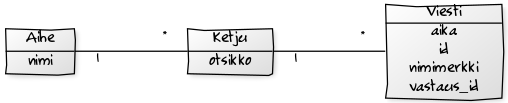
\includegraphics[width=\textwidth]{6bd37a82}
\end{figure}
\subsection{Attribuutit}
\emph{Aihe.nimi}: Aiheen nimi merkkijonona, jonka pituus korkeintaan 255 merkkiä. \\
\emph{Ketju.otsikko}: Ketjun nimi  merkkijonona, jonka pituus korkeintaan 255 merkkiä. \\
\emph{Viesti.aika}: Viestin lähetysaika timestampina. \\
\emph{Viesti.id}: Viestin id kokonaislukuna. \\
\emph{Viesti.nimimerkki}: Lähettäjän nimimerkki merkkijonona, jonka pituus korkeintaan 255 merkkiä. \\
\emph{Viesti.vastaus\_id}: Vastattavan viestin id kokonaislukuna. \\
\emph{Viesti.sisältö}: Viestin sisältö merkkijonona, jonka pituus korkeintaan 1020 merkkiä. \\
\section{Tietokantakaavio}
\begin{figure}[h]
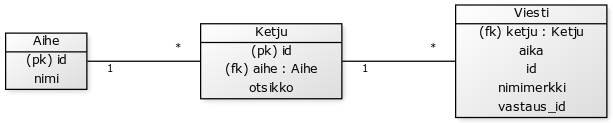
\includegraphics[width=\textwidth]{2ca63d43}
\end{figure}
\section{CREATE TABLE lausekkeet}
CREATE TABLE Aihe (id integer PRIMARY KEY, nimi varchar(255) NOT NULL); \\
CREATE TABLE Ketju (id integer PRIMARY KEY, aihe integer NOT NULL, otsikko varchar(255) NOT NULL, FOREIGN KEY(aihe) REFERENCES Aihe(id)); \\
CREATE TABLE Viesti (ketju integer NOT NULL, aika timestamp NOT NULL, id integer NOT NULL, nimimerkki varchar(255) NOT NULL, sisältö varchar(1020) NOT NULL, FOREIGN KEY(ketju) REFERENCES Ketju(id));
\section{Keskeisiä käyttötapauksia}
Listataan kaikki aiheet: \\
SELECT nimi FROM Aihe; \\\\
Listataan kaikki tiettyyn aiheeseen liittyvät ketjut: \\
SELECT K.otsikko FROM Aihe A, Ketju K WHERE A.id = K.aihe AND A.id = ?; \\\\
Listataan kaikki tiettyyn ketjuun liittyvät viestit: \\
SELECT Viesti FROM Ketju K, Viesti V WHERE K.id = V.ketju AND K.id = ?;
\end{document}
